% !TeX spellcheck = cs_CZ
\wikitextrule
\begin{example}\label{MAI:exam021} 
  Pro funkci z příkladu \ref{MAI:exam023} platí:
  \begin{align*}
    \sup_{x\in\realset}&=\frac{1}{x^2+1}=\max_{x\in\realset}=\frac{1}{x^2+1}=1;   \\
    \inf_{x\in\realset}&=\frac{1}{x^2+1}=0,
  \end{align*}
  tato funkce však nenabývá v definičním oboru $\realset$ nejmenší hodnoty, neboť je stále 
  $\dfrac{1}{x^2+1}>0$. To, že infimum je $0$, dokážeme takto: Zvolíme-li libovolně 
  $\varepsilon>0$, pak snadno zjistíme, že existuje $x$, pro něž 
  $\dfrac{1}{x^2+1}<\varepsilon$:
  \begin{align*}
    1                  &< \varepsilon(x^2+1) \\
    \frac{1}{\epsilon} &< x^2+1 \Rightarrow \sqrt{\frac{1}{\epsilon}-1} < x
  \end{align*} 
  
  {\centering
   \captionsetup{type=figure}
%   % !TeX spellcheck = cs_CZ
%Graf funkce $f(x):y=\dfrac{1}{1+x^2}$

\documentclass[11pt]{standalone}
\usepackage{xltxtra}
\usepackage[usenames,x11names]{xcolor}
\usepackage{tikz}
\usepackage{pgfplots}
  \pgfplotsset{compat=newest}
\usepackage{amsmath}

\begin{document}
  \begin{tikzpicture}[thick,scale=0.7, every node/.style={transform shape}]
    \begin{axis}[
      xmin = -4.2, xmax = 4.5, ymin = 0, ymax = 1.3,  % osy
      domain = -4:4,
      restrict y to domain=0:1,
  %    unit vector ratio=1 1 1,  % axis equal
      grid = major,   % both
      grid style={line width=.1pt, draw=gray!20},
      major grid style={dashed, line width=.2pt, draw=gray!40},
      minor tick num=5,
      clip = true,
      clip mode=individual,
  %    /pgfplots/xtick={-2,-1,1,2}, % make steps of length 0.2
      axis x line = middle,
      axis y line = middle,
      xlabel={\(x\)}, ylabel={\(y\)},
      enlarge y limits={rel=0.07},
      enlarge x limits={rel=0.07},
    ]
    
      \addplot[color=Gold3, samples=200, smooth, ultra thick, unbounded coords=jump, no markers] 
         gnuplot{1/sqrt(1+x^2)};  
    \end{axis}
  \end{tikzpicture}
\end{document} 
   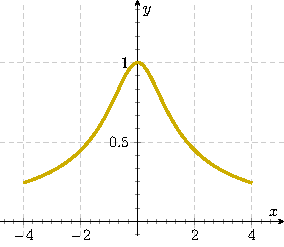
\includegraphics[width=0.5\linewidth]{mai_fig009.pdf}
   \captionof{figure}{Graf funkce $f(x):y=\dfrac{1}{1+x^2}$}
   \label{mai:fig009}
  \par}
  
  Neexistuje tedy kladné číslo, jež by bylo dolní mezí množiny funkčních hodnot, takže infimum je 
  $0$. Graf funkce $f$ je na obr. \ref{mai:fig009}.
\end{example}